\chapter{The LHCb experiment}
\label{ref:detector}

The LHCb experiment is dedicated for $b$ and $c$-physics precision measurements.
It is one of the four large experiments
(CMS, ATLAS, ALICE, LHCb) at the Large Hadron Collider (LHC),
a superconducting circular $pp$ collider, built and managed by
the European Organization for Nuclear Research (CERN),
with a center of mass energy
$\sqrt{s} = 13$~TeV during its run 2 (2016--2018) operation period.

Located 100 meters underground at Franco-Swiss border,
the LHCb detector,
shown in \cref{fig:lhcb-detector},
is a forward only spectrometer covering the pseudorapidity\footnote{
    Defined as the following:
    $\eta \equiv -\ln\left[\tan\left(\frac{\theta}{2}\right)\right]$,
    with $\theta$ the angle between the 3-momentum of a particle
    and the positive direction of the beam axis.
}
range $1.9 < \eta < 4.9$.
% coverage of bbbar
The unusual geometry of the LHCb detector
(as opposed to $4\pi$ detectors with full solid angle coverage,
for example the other three large experiments at the LHC)
is largely driven by the \bbbar production mechanism at the LHC:
the dominate production mode is gluon fusion in which case the momenta of the
incoming partons are highly asymmetric in the lab frame.
As a result, the \bbbar center of mass is boosted either forward or backward
in the beam direction \cite{Altarelli_2008}.
Simulation of \bbbar production angular distribution,
shown in \cref{fig:bbbar-prod-angular},
confirms the claim above.
With just about 4\% solid angle coverage,
the LHCb detector efficiently and economically reconstructs about 20\%
of all produced \bbbar pairs \cite{Belyaev_2021}.

% luminosity run 1+2
At the designed LHC luminosity, multiple $pp$ collisions happen within the
same bunch crossing (an effect called ``pile up'')
which greatly complicates \bbbar production and event reconstruction because
the event\footnote{
    An event is defined as \emph{everything} produced in a single bunch
    crossing.
} is significantly more \emph{busy}
(compared to events with single $pp$ collision)
\cite{Altarelli_2008}.
To maintain the luminosity at optimal values for LHCb,
a technique termed \emph{luminosity levelling} is implemented to dynamically
\emph{defocus} beams by offsetting them in the transverse direction based
on reported LHC instantaneous luminosity
\cite{https://doi.org/10.5170/cern-2014-004.183}.
%%%%
Over the course of run 1 and 2 operation periods, LHCb recorded a total
integrated luminosity of $\sim 8.7$~fb$^{-1}$
\cite{LHCb_lumi},
an unprecedented number for $b$-physics.

The rest of chapter provides a brief introduction for the subdetectors of the
LHCb detector relevant for this analysis, grouped based on the main utility of
each subdetector.
An overview of reconstruction of charged particles is provided in
\cref{ref:detector:tracking};
the particle identification is described in \cref{ref:detector:pid};
the basics of trigger implementation is explained in
\cref{ref:detector:trigger}.

\begin{figure}[!htb]
    \centering
    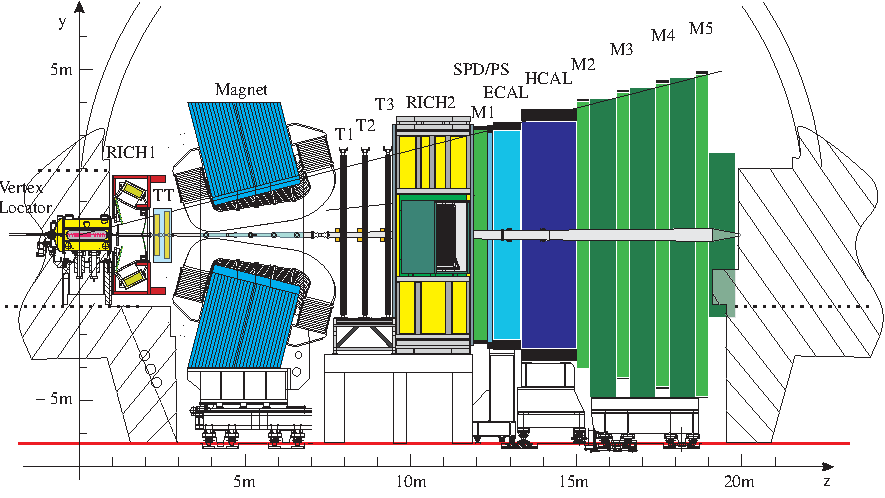
\includegraphics[width=0.95\textwidth]{./figs-detector/lhcb_detector_view.pdf}
    \caption{The LHCb detector.}
    \label{fig:lhcb-detector}
\end{figure}

\begin{figure}[!htb]
    \centering
    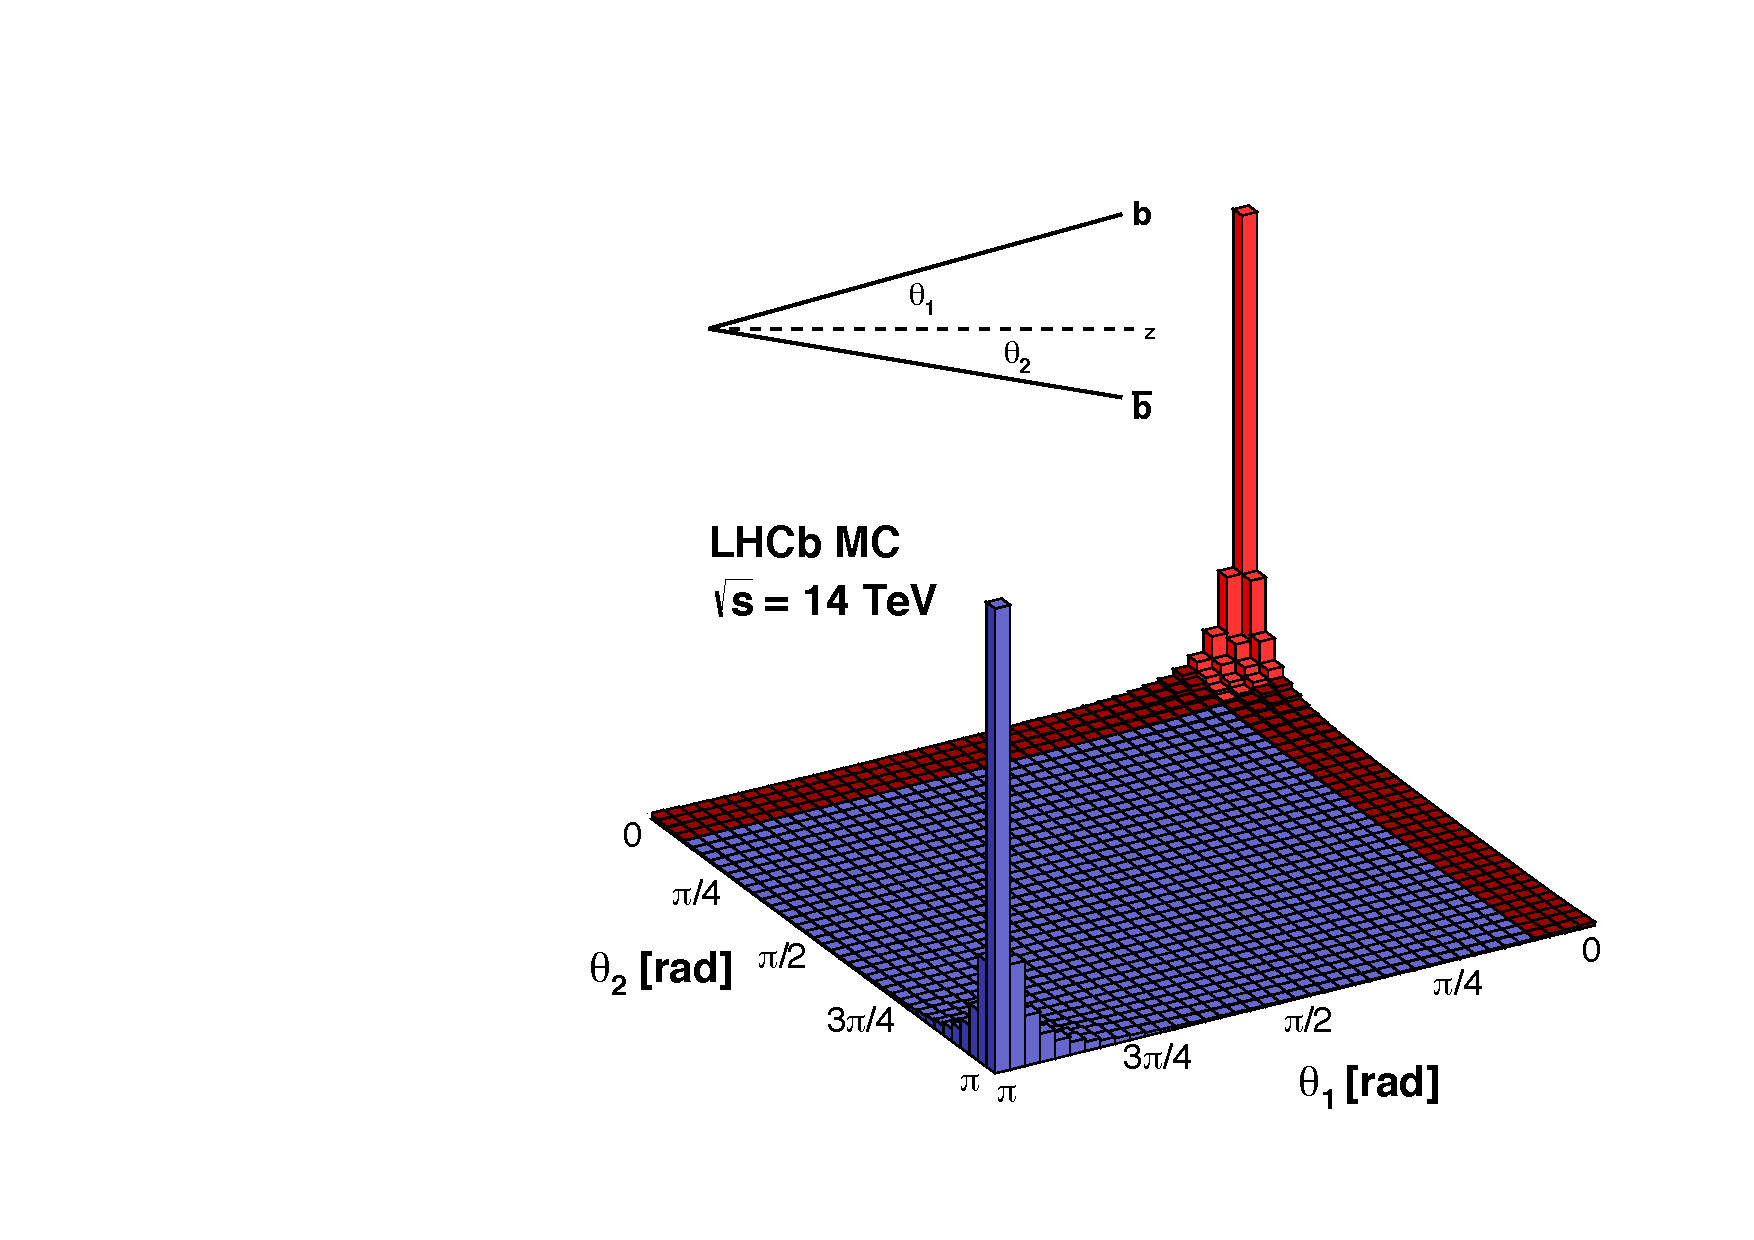
\includegraphics[width=0.6\textwidth]{./figs-detector/14_rad_acc_scheme_right.pdf}
    \caption{
        Simulated \bbbar production angular distribution at $\sqrt{s} = 14$ GeV.
        Taken from \cite{LHCb_bb_prod_angle}.
    }
    \label{fig:bbbar-prod-angular}
\end{figure}


\section{Reconstruction of charged particles}
\label{ref:detector:tracking}


\section{Particle identification}
\label{ref:detector:pid}


\section{Trigger}
\label{ref:detector:trigger}
